\documentclass[11pt,a4paper]{article}\usepackage[]{graphicx}\usepackage[]{xcolor}
% maxwidth is the original width if it is less than linewidth
% otherwise use linewidth (to make sure the graphics do not exceed the margin)
\makeatletter
\def\maxwidth{ %
  \ifdim\Gin@nat@width>\linewidth
    \linewidth
  \else
    \Gin@nat@width
  \fi
}
\makeatother

\definecolor{fgcolor}{rgb}{0.345, 0.345, 0.345}
\newcommand{\hlnum}[1]{\textcolor[rgb]{0.686,0.059,0.569}{#1}}%
\newcommand{\hlstr}[1]{\textcolor[rgb]{0.192,0.494,0.8}{#1}}%
\newcommand{\hlcom}[1]{\textcolor[rgb]{0.678,0.584,0.686}{\textit{#1}}}%
\newcommand{\hlopt}[1]{\textcolor[rgb]{0,0,0}{#1}}%
\newcommand{\hlstd}[1]{\textcolor[rgb]{0.345,0.345,0.345}{#1}}%
\newcommand{\hlkwa}[1]{\textcolor[rgb]{0.161,0.373,0.58}{\textbf{#1}}}%
\newcommand{\hlkwb}[1]{\textcolor[rgb]{0.69,0.353,0.396}{#1}}%
\newcommand{\hlkwc}[1]{\textcolor[rgb]{0.333,0.667,0.333}{#1}}%
\newcommand{\hlkwd}[1]{\textcolor[rgb]{0.737,0.353,0.396}{\textbf{#1}}}%
\let\hlipl\hlkwb

\usepackage{framed}
\makeatletter
\newenvironment{kframe}{%
 \def\at@end@of@kframe{}%
 \ifinner\ifhmode%
  \def\at@end@of@kframe{\end{minipage}}%
  \begin{minipage}{\columnwidth}%
 \fi\fi%
 \def\FrameCommand##1{\hskip\@totalleftmargin \hskip-\fboxsep
 \colorbox{shadecolor}{##1}\hskip-\fboxsep
     % There is no \\@totalrightmargin, so:
     \hskip-\linewidth \hskip-\@totalleftmargin \hskip\columnwidth}%
 \MakeFramed {\advance\hsize-\width
   \@totalleftmargin\z@ \linewidth\hsize
   \@setminipage}}%
 {\par\unskip\endMakeFramed%
 \at@end@of@kframe}
\makeatother

\definecolor{shadecolor}{rgb}{.97, .97, .97}
\definecolor{messagecolor}{rgb}{0, 0, 0}
\definecolor{warningcolor}{rgb}{1, 0, 1}
\definecolor{errorcolor}{rgb}{1, 0, 0}
\newenvironment{knitrout}{}{} % an empty environment to be redefined in TeX

\usepackage{alltt}
\usepackage{alltt}
\usepackage[utf8]{inputenc}
\usepackage[T1]{fontenc}
\usepackage{listings}
\usepackage{marvosym}
\usepackage{mathtools, amsthm, amssymb}
\usepackage[english]{babel}
\usepackage{enumitem}
\usepackage[hidelinks]{hyperref}
\usepackage{amsmath}
\usepackage{mathpazo}
\usepackage{graphicx}
\usepackage{siunitx}
\usepackage{geometry}
\usepackage{dirtytalk}
\usepackage{xcolor}
\usepackage{mathtools}
\usepackage{graphicx}
\usepackage{graphics}
\usepackage{caption}
\usepackage{colortbl}
\usepackage{subcaption}
\usepackage{tabularx}
\usepackage{makecell}
\usepackage[toc,page]{appendix}
\usepackage{xurl}


\newcommand{\RomanNumeralCaps}[1]
    {\MakeUppercase{\romannumeral #1}}


\DeclareMathOperator\erf{erf}
\newtheorem{definition}{Definition}

\newtheorem{theorem}{Theorem}
\IfFileExists{upquote.sty}{\usepackage{upquote}}{}
\IfFileExists{upquote.sty}{\usepackage{upquote}}{}
\begin{document}
	
	
	\begin{titlepage} 
		\newcommand{\HRule}{\rule{\linewidth}{0.5mm}} 
		
		\center 
		
		
		
		\HRule\\[0.4cm]
		
		{\huge\bfseries Project Part \RomanNumeralCaps{2}

			
			Data Mining}\\[0.4cm] 
		
		\HRule\\[1.5cm]
		
		
		\begin{minipage}{0.4\textwidth}
			\begin{flushleft}
				\large
				
				Julia Kończal
				
				Piotr Zieleń 
			\end{flushleft}
		\end{minipage}
		~
		\begin{minipage}{0.4\textwidth}
			\begin{flushright}
				\large
				group: Wednesday 13.15
				
				
				
				
				
				
				
				
				
			\end{flushright}
		\end{minipage}
		
		
		
		\vfill\vfill\vfill 	\vspace{400px}
		
		
		{\large \today} 
		
		\vfill 
		
	\end{titlepage}
	
	\newpage
	
	\newpage
	
	\tableofcontents
	\newpage
	\section{Introduction}

	
	\subsection{Our dataset}
	Our dataset comes from \url{https://archive.ics.uci.edu/dataset/10/automobile}. The data consists of 204 instances and contains 26 features (categorical, integer, real). The automobile dataset under consideration serves as a comprehensive repository of information related to various aspects of the automotive industry. Ranging from vehicle specifications and performance metrics to market trends and historical data, this dataset encapsulates a wealth of information crucial for understanding the dynamics of the automotive sector. Analyzing this dataset can provide valuable insights into factors influencing vehicle design, consumer preferences, and industry trends, making it an invaluable resource for researchers, analysts, and enthusiasts alike.
	
	\subsection{Problem description and research questions}
	
The automotive industry faces the challenge of effectively analyzing vast datasets containing diverse information about vehicle attributes, performance metrics, and safety features. Efficiently extracting valuable insights from these datasets is crucial for market research, product development, and decision-making processes within the industry.

To address this challenge, our project focuses on utilizing data mining methods to perform a comprehensive analysis of automobile data. The primary objective is to gain a deeper understanding of the underlying patterns, trends, and relationships within the dataset, ultimately aiding in decision-making processes and strategic planning within the automotive sector.

Specifically, we aim to tackle the following aspects:
\begin{enumerate}
\item Cluster analysis --- The first part of our project involves conducting cluster analysis on the automobile dataset. By applying clustering algorithms such as K-means, Partitioning Around Medoids (PAM), Agglomerative Nesting (AGNES), and Divisive Analysis (DIANA), we seek to identify natural groupings or clusters of vehicles based on their attributes. This analysis will help uncover distinct segments within the automotive market and provide insights into consumer preferences, market trends, and competitive landscapes.
\item Dimension reduction and visualization --- In the second part of the project, we will explore the application of multidimensional scaling (MDS) as a dimension reduction method. MDS will be used to visualize the relationships between vehicles in a lower--dimensional space, allowing for a clearer understanding of similarities and differences among vehicles based on their attributes. The reduced--dimensional representation obtained through MDS will be leveraged in conjunction with classification and cluster analysis to enhance the interpretability and accuracy of our results.
\item Performance evaluation and comparison --- Throughout the project, we will emphasize performance evaluation and comparison of the data mining methods and algorithms employed. We will assess the effectiveness of each clustering algorithm in identifying meaningful clusters within the dataset and evaluate the practical usefulness of the dimension reduction method in improving the analysis outcomes. Quality assessment metrics will be utilized to measure the performance of each method, enabling us to draw comprehensive conclusions regarding their applicability and effectiveness.
By addressing these aspects, our project aims to provide valuable insights into the practical utility of data mining techniques in the context of automobile data analysis. The outcomes of this analysis will facilitate informed decision-making processes and strategic planning within the automotive industry, ultimately contributing to enhanced competitiveness and innovation in the market.
\end{enumerate}

In the project we want to answer the following questions:
\begin{enumerate}
\item How does clustering performance vary across different methods and numbers of clusters?
\item What impact does multidimensional scaling (MDS) dimensionality reduction have on clustering results?
\item What is the effect of feature selection or dimensionality reduction techniques on the performance of classification algorithms?
\end{enumerate}
	\subsection{Methods and algorithms used in the project}
	We utilized R programming language for the implementation of this project. The libraries and versions that we used to prepare the whole project are: dplyr (1.1.2), mice (3.16.0), kableExtra (1.3.4), naniar(1.0.0), VIM (6.2.2), ggplot2 (3.4.3), gridExtra (2.3), ie2misc (0.9.1), EnvStats (2.8.1), corrplot (0.92), ggpubr (0.6.0), knitr (1.43), patchwork (1.1.3), caret (6.0-94), tidyr (1.3.0), arules (1.7-7), MASS (7.3-60), janitor (2.2.0), class (7.3-22), rpart (4.1.19), rpart.plot (3.1.1), rattle (5.5.1), e1081 (1.7-13), factoextra (1.0.7), cluster (2.1.4), clValid (0.7).


	
	The methods and other important terms that we utilized during preparation of the project:
	\begin{itemize}
	
\item K--means --- an unsupervised machine learning algorithm used for clustering data into groups or clusters based on similarity. It aims to partition data points into $K$ clusters where each data point belongs to the cluster with the nearest mean (centroid). The algorithm iteratively assigns data points to the nearest centroid and then updates the centroids based on the mean of the data points assigned to each cluster. This process continues until convergence, where the centroids no longer change significantly, or a specified number of iterations is reached. K--means has some limitations, such as sensitivity to the initial placement of centroids, the need to specify the number of clusters ($K$) beforehand, and its susceptibility to outliers. Various techniques, such as multiple initializations and evaluation metrics like the silhouette score, can be employed to mitigate these limitations. Additionally, more advanced variations of K-means, such as K-means++, address some of these challenges by improving the initialization step.

\item Partitioning Around Medoids (PAM) --- a clustering algorithm similar to K-means, but it uses medoids instead of centroids to define clusters. Medoids are representative data points within each cluster, whereas centroids are the mean points of the data. PAM has some advantages over K--means, such as being more robust to noise and outliers since it uses actual data points as representatives (medoids) instead of centroids, which can be influenced by outliers, it allows using qualitative features during clustering. However, PAM tends to be computationally more expensive than K--means, especially as the size of the dataset increases, because it involves calculating pairwise dissimilarities between data points.

\item Agglomerative Nesting (AGNES) --- a hierarchical clustering algorithm that operates by recursively merging clusters of data points into larger clusters based on their similarity. Unlike K--means and PAM, which require specifying the number of clusters beforehand, AGNES does not require specifying the number of clusters in advance. AGNES has several advantages, including its ability to handle any shape of clusters, its interpretability through dendrogram visualization, and its lack of dependence on the number of clusters. However, it can be computationally expensive, especially for large datasets, due to its pairwise distance calculations.

\item Divisive Analysis (DIANA) --- a hierarchical clustering algorithm, similar to AGNES, but it operates in a divisive manner. While AGNES starts with individual data points and iteratively merges them into clusters, DIANA begins with all data points in a single cluster and recursively divides them into smaller clusters. DIANA has similar advantages and disadvantages to AGNES. It can handle arbitrary cluster shapes, provides interpretability through dendrogram visualization, and does not require specifying the number of clusters in advance. However, it can be computationally expensive for large datasets due to its pairwise distance calculations.

\item Multidimensional Scaling (MDS) --- a technique used in statistics and data analysis to visualize the similarity or dissimilarity between data points in a high-dimensional space by projecting them into a lower-dimensional space. MDS aims to preserve the pairwise distances or dissimilarities between data points as much as possible in the lower-dimensional representation, allowing for easier interpretation and visualization of complex relationships among the data. MDS can be applied in various fields, including psychology, marketing, biology, and geographic information systems (GIS), to analyze and visualize complex data relationships. It is particularly useful when dealing with high-dimensional data or when the relationships between data points are not readily apparent in the original space.

\item average Silhouette width - also known as the mean Silhouette score, is a metric used to evaluate the quality of a clustering algorithm. It measures how well each data point fits within its assigned cluster compared to other clusters. A higher Silhouette score indicates better-defined clusters, with data points being closer to other points in the same cluster and farther away from points in other clusters.

\item average linkage --- in this method the distance between two clusters is calculated as the average distance between all pairs of points in the two clusters. It considers the mean distance between all points in one cluster to all points in the other cluster. Average linkage tends to produce more balanced and compact clusters compared to single or complete linkage and is less sensitive to outliers.
 \item complete linkage --- in this method the distance between two clusters is calculated as the maximum distance between any two points in the two clusters. It considers the maximum distance between any point in one cluster and any point in the other cluster. Complete linkage tends to produce compact, spherical clusters but can be sensitive to noise and outliers.
 \item single linkage --- this method measures the distance between two clusters as the shortest distance between any two points in the two clusters. It considers only the minimum distance between any point in one cluster and any point in the other cluster. Single linkage tends to produce long, elongated clusters, as it is sensitive to outliers and tends to merge clusters based on nearby points.
	
	\end{itemize}
	
	

	

	
	

	

	

	




	



	

	

	


	

	

	


	

	

	
	



	
	

	
	



	
	

	



	


	


	

	

	

	
	


	

	


	

	

	

	

	

	


	


	

	

	



	




	\section{Clustering}\label{sec:clustering}
	In this part of the project, we will attempt to cluster our dataset independently of their originally corresponding class. The objective is to explore whether there are inherent properties within the data and to observe how clustering methods, specifically unsupervised learning, align with the previously considered classification methods.
		
	Clustering--based methods are those, which search for the data, having similar features and grouping them to the same class. Those methods do not use originally assigned classes during learning process. There exist a lot of types of clustering methods, in this project we will consider: k--means (for quantitative features), Partitioning Around Medoids (PAM), Agglomerative Nesting (AGNES) and Divisive Analysis (DIANA) methods.
	
	Before we will perform clusterisation, we have to decide, how many clusters are in our dataset. Using external information, we know that our class label consists of 5 unique values, but from the practical point of view, there can be such a situation, that the real number of clusters is unknown. So we will use average Silhouette width to assess, which number of clusters will turn out to be the best. The external information (number of unique variables in our class label) we will use to evaluate, if the above considered methods provided reasonable value of number of the clusters.
	
	\subsection{Data preparation}
	
	When considering clusterization algorithms, we prepare the data in the same rule as for classification methods, but we skip one--hot encoding. In case of unsupervised learning, we don't consider train and test sets, so we have to merge our before considered samples. 
	

	
	\subsection{Number of clusters selection}\label{sec:optimal_cluster_number}
	We want to assess which number of clusters will be the best choice for each considered clustering partitioning method. To do this, we will consider a range from 1 to 10 clusters and for each considered clustering method, we will assess which of them has the best score.
	
	In case of k--means it is allowed use only quantitative data, so in our case we have to restrict only to numerical attributes.
	
\begin{knitrout}
\definecolor{shadecolor}{rgb}{0.969, 0.969, 0.969}\color{fgcolor}\begin{figure}
\includegraphics[width=\maxwidth]{figure/kmeans_number_of_clusters-1} \caption[Results of elbow and silhouette method in order to choose optimal number of clusters for k-means algorithm]{Results of elbow and silhouette method in order to choose optimal number of clusters for k-means algorithm}\label{fig:kmeans_number_of_clusters}
\end{figure}

\end{knitrout}
	
	In figure \ref{fig:kmeans_number_of_clusters} we can see results for "elbow" (left chart) and "silhouette" (right chart) methods for selecting optimal number of clusters in considered dataset. The elbow method is a naive approach and selecting optimal number of clusters depends on the interpretation. And in general you select the number, for which the within-cluster dispersion stops rapidly decreasing, and increasing the number of clusters does not yield much improvement. By interpreting only the chart it is really hard to find a trade-off between the obtained results and selecting number of clusters, because we would like to have quite small number clusters. By looking at the results for silhouette method we can see, and it is also marked by dash line, that the best number of cluster is equal to 2. When interpreting the results we decide that for k--means algorithm we will assume number of clusters equal to 2.
	
	In case of PAM clustering method, firstly we have to determine dissimilarity matrix between objects. In order to do this, we will use Gower's formula. It is a method used to calculate the dissimilarity between pairs of objects or data points in a mixed data set. Unlike traditional distance metrics that assume homogeneity of data types (e.g., numerical or categorical), Gower's formula can handle a mix of different types of variables, including numerical, categorical, and ordinal. The formula takes into account the nature of each variable type and computes dissimilarities accordingly, providing a more comprehensive measure of dissimilarity between objects. This makes Gower's formula particularly useful in multidimensional scaling, clustering, and other data analysis techniques where heterogeneous data types are common.

	
	To assess which number of clusters will be the best choice, we will calculate average silhouette width, and we will choose the number, with the largest value.
	

	
\begin{knitrout}
\definecolor{shadecolor}{rgb}{0.969, 0.969, 0.969}\color{fgcolor}\begin{figure}
\includegraphics[width=\maxwidth]{figure/pam_silhouette-1} \caption[Results of average silhouette width for PAM clustering method]{Results of average silhouette width for PAM clustering method}\label{fig:pam_silhouette}
\end{figure}

\end{knitrout}
	
	In figure \ref{fig:pam_silhouette} we can see results of average silhouette width for PAM clustering method, for considered range of cluster numbers. As we can see the largest value of average width is obtained for 2 clusters and the value in this case is equal to 0.3803213, so for PAM algorithm we will choose this number as an optimal value.
	Now we will consider hierarchical clustering methods --- Aglomerative Nesting (AGNES) and Divisite Analysis (DIANA). In case of AGNES we will consider three linkage methods: average, complete, single. In order to assess which number of clusters perform the best, we will use average silhouette width.
	

	

	

	
\begin{knitrout}
\definecolor{shadecolor}{rgb}{0.969, 0.969, 0.969}\color{fgcolor}\begin{figure}
\includegraphics[width=\maxwidth]{figure/agnes_silhouette-1} \caption[Results of average silhouette width for AGNES clustering method for average, single and complete linkage]{Results of average silhouette width for AGNES clustering method for average, single and complete linkage}\label{fig:agnes_silhouette}
\end{figure}

\end{knitrout}
	
	In the figure \ref{fig:agnes_silhouette} we can see average silhouette width for number of clusters in range from 1 to 10 and for three linkage methods: average, single and complete and as we may see for average and simple linkage methods, the largest value is obtained for 2 clusters, and are equal respectively 0.366675, 0.2811714. In case of complete linkage, the largest value is equal to 0.3092302 and is obtained for 3 clusters.
	
	The last considered clusterisation method is Divisive Analysis. Let's check which number of clusters will be optimal for this method:
	

	
\begin{knitrout}
\definecolor{shadecolor}{rgb}{0.969, 0.969, 0.969}\color{fgcolor}\begin{figure}
\includegraphics[width=\maxwidth]{figure/diana_silhouette-1} \caption[Results of average silhouette width for DIANA clustering method]{Results of average silhouette width for DIANA clustering method}\label{fig:diana_silhouette}
\end{figure}

\end{knitrout}
	
	For DIANA algorithm the optimal number of clusters is also equal to 2 (as we may see in figure \ref{fig:diana_silhouette}) like for a majority of considered methods, and the average silhouette width for this number of clusters is equal to 0.3260946.
	
	While most clustering methods yielded an optimal number of clusters equal to 2 based on the average silhouette width, AGNES with the complete linkage method deviated from this trend, suggesting the presence of a more complex data structure that requires additional clusters for accurate representation.
	
	Despite the consistency in the optimal number of clusters across various methods, external knowledge indicating the presence of 5 clusters highlights the importance of contextual understanding and domain expertise in interpreting clustering results. This underscores the need for a holistic approach that integrates both data-driven insights and domain-specific knowledge.
	
	In the upcoming subsections, we will further evaluate the quality of clustering using a combination of external and internal indices, providing a comprehensive assessment of clustering performance and its relevance to the practical problem at hand.
	
	\subsection{K--means}
	
	K--means clustering is popular clustering method, but as one important remark is that it works only for quantitative features. In subsection \ref{sec:optimal_cluster_number} we have selected 2 as an optimal number of clusters for this method. Now we will assess quality of the k--means clustering algorithm.
	
\begin{knitrout}
\definecolor{shadecolor}{rgb}{0.969, 0.969, 0.969}\color{fgcolor}\begin{kframe}
\begin{verbatim}
##   cluster size ave.sil.width
## 1       1  132          0.40
## 2       2   69          0.21
##   cluster size ave.sil.width
## 1       1   37          0.23
## 2       2   15          0.16
## 3       3   52          0.16
## 4       4   54          0.34
## 5       5   43          0.13
\end{verbatim}
\end{kframe}\begin{figure}
\includegraphics[width=\maxwidth]{figure/silhouette_kmeans25-1} \caption[Silhouette indices for k-means clustering method, for 2 and 5 clusters]{Silhouette indices for k-means clustering method, for 2 and 5 clusters}\label{fig:silhouette_kmeans25}
\end{figure}

\end{knitrout}
	
	In the figure \ref{fig:silhouette_kmeans25} we can see silhouette plots for k--means algorithm, for 2 (chart at the top) and for 5 clusters (chart at the bottom). Dashed lines indicate the average silhouette width (the exact value is written in the titles of charts). 
%	As we can see in the chart for 2 clusters, more observations belongs to cluster "1" and anyone of them were wrongly assigned. For cluster "2", there are some incorrectly assigned observations, because as we may see on the right side of the chart, some values are negative.
	
	For the case of 2 clusters, the silhouette plot (and output of R code) reveals that one cluster ("1") contains a majority of the observations, with no misattributed observations. However, cluster "2" exhibits some misattributed observations, as indicated by the presence of negative silhouette widths. This suggests that the separation between clusters is not optimal, leading to misclassifications for some data points.
	
%	In case of 5 clusters (below chart), we may see, that in all, apart from "4" (blue one) clusters, there are few misattributes observations. The "4" cluster is the biggest one, and the silhouette width for this cluster is for sure the largest (we can see that by interpreting the chart).

In contrast, when considering 5 clusters, the silhouette plot indicates a more balanced distribution of observations across clusters, except for cluster "4," which appears to be the largest. Despite its size, cluster "4" exhibits a high silhouette width, suggesting that the intra-cluster cohesion is strong. However, the presence of misattributed observations in other clusters indicates potential overlaps or insufficient separation between clusters.
	
Now, let us compare cluster labels with the actual classes. We will utilize external knowledge to assess quality. In order to do this, we will create a contingency table and then match the cluster and actual class labels to find the largest value.
	
\begin{knitrout}
\definecolor{shadecolor}{rgb}{0.969, 0.969, 0.969}\color{fgcolor}\begin{kframe}
\begin{verbatim}
## Direct agreement: 3 of 5 pairs
## Iterations for permutation matching: 2 
## Cases in matched pairs: 49.75 %
##    1    2    3    4    5 
## "-1"  "2"  "0"  "1"  "3"
\end{verbatim}
\end{kframe}
\end{knitrout}
	
As we can see above, after matching classes, we obtained nearly 50\% agreement between the actual and cluster class labels. It suggests moderate alignment between the clustering results and the true class labels. While this level of agreement indicates some level of clustering accuracy, further analysis may be necessary to explore potential factors contributing to misclassifications and to improve the overall clustering performance. 
	
	\subsection{Partitioning Around Medoids (PAM)}
	
	PAM algorithm is more general than the k--means. This method works for both types of data: quantitative and qualitative. In subsection \ref{sec:optimal_cluster_number} we have calculated, based on silhouette average width, that the optimal number of clusters is equal to 2. Let us generate the silhouette plot for this number and for 5 clusters, to compare results with actual class labels.
	
\begin{knitrout}
\definecolor{shadecolor}{rgb}{0.969, 0.969, 0.969}\color{fgcolor}\begin{kframe}
\begin{verbatim}
##   cluster size ave.sil.width
## 1       1   75          0.25
## 2       2  126          0.46
##   cluster size ave.sil.width
## 1       1   38          0.18
## 2       2   65          0.28
## 3       3   37          0.28
## 4       4   44          0.30
## 5       5   17          0.28
\end{verbatim}
\end{kframe}\begin{figure}
\includegraphics[width=\maxwidth]{figure/silhouette_pam25-1} \caption[Silhouette indices for PAM clustering method, for 2 and 5 clusters]{Silhouette indices for PAM clustering method, for 2 and 5 clusters}\label{fig:silhouette_pam25}
\end{figure}

\end{knitrout}
	
	In the figure \ref{fig:silhouette_pam25} we can see silhouette plots for PAM algorithm. Upper chart corresponds to 2 clusters and bottom --- to 5. When considering optimal, for this method, number of clusters, conclusions are similar as in case of k--means (\ref{fig:silhouette_kmeans25}). The bigger cluster has no incorrectly assigned observations, but the smaller one have 6 wrong misattributed ones. We can see, that for bigger cluster more than $\frac{1}{3}$ observations have silhouette index larger than 0.5, this implicates that they are quite well assigned, because, the closer the silhouette index to 1 is, the better.
	
	For the true number of clusters --- 5, we can see that each cluster consists of few incorrectly assigned observations. We can easily see that cluster "5" is the smaller one, and "2" --- the biggest one. Other clusters have quite similar size (by interpreting the chart).
	
	Similar trends to those observed with k--means clustering are evident. Despite the differences in algorithmic approach, both methods exhibit clusters with varying degrees of misattributed observations. This highlights the importance of thorough evaluation and comparison of clustering algorithms to identify the most suitable approach for a given dataset.
	
\begin{knitrout}
\definecolor{shadecolor}{rgb}{0.969, 0.969, 0.969}\color{fgcolor}\begin{kframe}
\begin{verbatim}
## Direct agreement: 1 of 5 pairs
## Iterations for permutation matching: 24 
## Cases in matched pairs: 45.77 %
##    1    2    3    4    5 
##  "3"  "0" "-1"  "1"  "2"
\end{verbatim}
\end{kframe}
\end{knitrout}
	
	Above, we observe the results for matching cluster and real classes. In this case, the agreement value is 45.77\%, which is noteworthy as it is smaller than in the case of k-means, where only quantitative features were considered. It suggests that while PAM may offer greater flexibility with mixed data types, it may not always result in as accurate clustering outcomes. 
	
	\subsection{Agglomerative Nesting (AGNES)}
In this subsection, we will delve into the AGNES clustering algorithm. We have opted not to analyze all three linkage methods but focus on the complete linkage method, as it yields an optimal number of clusters equal to 3. As a hierarchical clustering method, AGNES allows for visualization through dendrograms.
	
\begin{knitrout}
\definecolor{shadecolor}{rgb}{0.969, 0.969, 0.969}\color{fgcolor}\begin{kframe}
\begin{verbatim}
##   cluster size ave.sil.width
## 1       1   60          0.27
## 2       2  121          0.41
## 3       3   20          0.23
##   cluster size ave.sil.width
## 1       1   53          0.18
## 2       2   90          0.03
## 3       3   31          0.42
## 4       4    7          0.55
## 5       5   20          0.11
\end{verbatim}
\end{kframe}\begin{figure}
\includegraphics[width=\maxwidth]{figure/silhouette_agnes35-1} \caption[Silhouette indices for AGNES clustering method, with complete linkage method, for 3 and 5 clusters]{Silhouette indices for AGNES clustering method, with complete linkage method, for 3 and 5 clusters}\label{fig:silhouette_agnes35}
\end{figure}

\end{knitrout}
	
\begin{knitrout}
\definecolor{shadecolor}{rgb}{0.969, 0.969, 0.969}\color{fgcolor}\begin{figure}
\includegraphics[width=\maxwidth]{figure/dendrograms_agnes-1} \caption[Dendrograms for AGNES clustering method, with complete linkage, for 3 (upper chart) and 5 (bottom chart) clusters]{Dendrograms for AGNES clustering method, with complete linkage, for 3 (upper chart) and 5 (bottom chart) clusters}\label{fig:dendrograms_agnes}
\end{figure}

\end{knitrout}
	
	In the figure \ref{fig:silhouette_agnes35} we can see silhouette plots for AGNES clustering methods, with complete linkage, for 3 (upper chart) and 5 (bottom chart) clusters. In the titles there are values of average silhouette width for observed cases. When examining the case of 3 clusters, we observe that each cluster contains a few incorrectly assigned observations. Additionally, there appears to be a notable discrepancy in cluster sizes, with significant variations between the largest and smallest clusters.
	
	The silhouette plot for 5 clusters case looks quite interesting. We can see that almost half of the observations that belong to the cluster "2", is wrongly assigned. Moreover, clusters 4 and 5 exhibit a peculiar pattern, suggesting potential forced separation. This analysis suggests that opting for 5 clusters may not be an optimal choice for the considered method.
	
The misclassification of nearly half of the observations in cluster "2" suggests potential challenges in accurately capturing the underlying data structure or distinguishing between closely related clusters. This highlights the need for fine-tuning clustering parameters or exploring alternative algorithms to improve clustering accuracy.	

	
\begin{knitrout}
\definecolor{shadecolor}{rgb}{0.969, 0.969, 0.969}\color{fgcolor}\begin{kframe}
\begin{verbatim}
## Direct agreement: 0 of 5 pairs
## Iterations for permutation matching: 120 
## Cases in matched pairs: 35.82 %
##    1    2    3    4    5 
##  "3"  "0"  "1"  "2" "-1"
\end{verbatim}
\end{kframe}
\end{knitrout}
	By matching clusters and real class labels, we got only 35.82\% agreement.
	
	Figure \ref{fig:dendrograms_agnes} shows dendrograms for 3 and 5 clusters, for AGNES clustering method with complete linkage. Labels, which are on x--axis  (not clearly visible), shows number of observations. In these charts we can see structures of the clusters. 
	
	\subsection{Divisive Analysis (DIANA)}
	
	Last considered clustering method is DIANA. In subsection \ref{sec:optimal_cluster_number}, we got, that based on average silhouette width, optimal number of cluster for this method is equal to 2. So we will analyse silhouette plots for 2 and 5 clusters (to compare with real class labels). DIANA is as an AGNES hierarchical clustering method, so we can make a dendrogram.
	
\begin{knitrout}
\definecolor{shadecolor}{rgb}{0.969, 0.969, 0.969}\color{fgcolor}\begin{kframe}
\begin{verbatim}
##   cluster size ave.sil.width
## 1       1  181          0.34
## 2       2   20          0.34
##   cluster size ave.sil.width
## 1       1   55          0.17
## 2       2   86          0.24
## 3       3   28          0.23
## 4       4   20          0.20
## 5       5   12          0.25
\end{verbatim}
\end{kframe}\begin{figure}
\includegraphics[width=\maxwidth]{figure/silhouette_diana25-1} \caption[Silhouette indices for DIANA clustering method, for 2 and 5 clusters]{Silhouette indices for DIANA clustering method, for 2 and 5 clusters}\label{fig:silhouette_diana25}
\end{figure}

\end{knitrout}
	
\begin{knitrout}
\definecolor{shadecolor}{rgb}{0.969, 0.969, 0.969}\color{fgcolor}\begin{figure}
\includegraphics[width=\maxwidth]{figure/dendrograms_diana-1} \caption[Dendrograms for DIANA clustering method, for 2 (upper chart) and 5 (bottom chart) clusters]{Dendrograms for DIANA clustering method, for 2 (upper chart) and 5 (bottom chart) clusters}\label{fig:dendrograms_diana}
\end{figure}

\end{knitrout}
	
	In the figure \ref{fig:silhouette_diana25} we can see as silhouette plots for DIANA clustering methods for 2 and 5 clusters. As we can see in case of 2 clusters, there is a large disproportion when considering cluster sizes. For the larger one belongs 0 observations, which are incorrectly assigned. The smaller one has no misattributed observations.
	
	For case of 5 clusters (bottom chart) we can see, that only "5" cluster has no misattributed observations. In total there are 0 incorrectly assigned observations. There are also quite significant disproportion when considering cluster sizes (at least when comparing the biggest one with three smallest ones).
	
	Figure \ref{fig:dendrograms_diana} shows dendrograms for DIANA clustering algorithms, for 2 and 5 clusters. In case of 2 clusters we may see mentioned earlier significant disproportion in case of cluster sizes.
	
\begin{knitrout}
\definecolor{shadecolor}{rgb}{0.969, 0.969, 0.969}\color{fgcolor}\begin{kframe}
\begin{verbatim}
## Direct agreement: 1 of 5 pairs
## Iterations for permutation matching: 24 
## Cases in matched pairs: 39.3 %
##    1    2    3    4    5 
##  "0"  "1"  "3" "-1"  "2"
\end{verbatim}
\end{kframe}
\end{knitrout}
	
	After matching clusters with real class labels we got almost 40\% agreement.
	
	\subsection{Results comparison}
	
	In this part of the project we have considered different clustering methods:
	\begin{itemize}
		\item Partitioning: k--means and Partitioning Around Medoids (PAM),
		\item Hierarchical: Agglomerative Nesting (AGNES) and Divisive Analysis (DIANA).
	\end{itemize}
	Firstly we checked what number of clusters will be optimal for all of considered algorithms, based on average silhouette width, and we got that 2 is the best choice for all methods, apart from AGNES with complete linkage, where for 3 clusters we got the largest value for average silhouette width. Then we analysed the methods for selected best number of choices and for 5 clusters, because of external knowledge. When comparing real class labels and cluster, after matching we got that partitioning clustering methods, provide better knowledge than hierarchical ones.
	
	At the end of this section we will report validation measures for clustering results. We will check internal separately for 2 and 5 clusters (avoiding case for 3 clusters). In terms of internal measures we will calculate:
	\begin{itemize}
		\item Connectivity --- Degree of connectedness of the clusters. The connectivity has a value between 0 and infinity and should be minimized,
		\item Silhouette width --- The Silhouette Width is the average of each observation's Silhouette value. The Silhouette value measures the degree of confidence in a particular clustering assignment and lies in the interval $[-1,1]$,
		\item Dunn ratio --- The Dunn Index is the ratio between the smallest distance between observations not in the same cluster to the largest intra-cluster distance. It has a value between 0 and infinity and should be maximized.
	\end{itemize}
	
\begin{knitrout}
\definecolor{shadecolor}{rgb}{0.969, 0.969, 0.969}\color{fgcolor}\begin{kframe}
\begin{verbatim}
##                  Score Method Clusters
## Connectivity 6.3988095  agnes        2
## Dunn         0.2250464  agnes        2
## Silhouette   0.4430771  agnes        2
\end{verbatim}
\end{kframe}
\end{knitrout}
	
	% Above we may see optimal results for internal measures, for 2 clusters. We considered: AGNES, k--means, DIANA and PAM clustering methods and for all of three measures we got that AGNES is the best choice, when considering internal measures (described before). 
	
	The optimal results for internal measures, particularly for 2 clusters, provide valuable insights into the performance of various clustering methods. In our analysis, which encompassed AGNES, k--means, DIANA, and PAM clustering methods, AGNES consistently emerged as the preferred choice based on internal evaluation metrics.

This finding underscores the effectiveness of AGNES in capturing the underlying structure of the data and generating cohesive clusters, as indicated by measures such as silhouette width.

The superiority of AGNES across multiple internal measures suggests its robustness and suitability for clustering tasks. Furthermore, the consistency of this outcome across different evaluation metrics lends credibility to the conclusion that AGNES is indeed the optimal choice for the given dataset and clustering objectives.

Overall, these findings highlight the importance of considering multiple evaluation criteria when selecting a clustering method and emphasize AGNES as a reliable option for generating high--quality clustering solutions in various analytical contexts.
	
\begin{knitrout}
\definecolor{shadecolor}{rgb}{0.969, 0.969, 0.969}\color{fgcolor}\begin{kframe}
\begin{verbatim}
##                   Score Method Clusters
## Connectivity 31.0202381  agnes        5
## Dunn          0.2312468  agnes        5
## Silhouette    0.3298561  diana        5
\end{verbatim}
\end{kframe}
\end{knitrout}
	
	% When considering 5 clusters, we got, that in case of Dunn ratio and connectivity, the best choice is AGNES and in case of Silhouette width --- DIANA. So in terms of internal measures hierarchical methods got better results.
	
	When considering 5 clusters, the analysis revealed notable differences in the performance of clustering methods across various internal measures. Specifically, the Dunn ratio and connectivity metrics favored AGNES, highlighting its ability to produce well-separated clusters with clear boundaries. On the other hand, DIANA outperformed other methods in terms of silhouette width, indicating its effectiveness in achieving high cluster cohesion and separation.
	
	
	
	Now we will check stability measures:
	\begin{itemize}
		\item The average proportion of non-overlap (APN),
		\item The average distance (AD),
		\item The average distance between means (ADM),
		\item The figure of merit (FOM).
	\end{itemize}
	The stability measures are a special version of internal measures which evaluate the stability of a clustering result by comparing it with the clusters obtained by removing one column at a time.
	
\begin{knitrout}
\definecolor{shadecolor}{rgb}{0.969, 0.969, 0.969}\color{fgcolor}\begin{kframe}
\begin{verbatim}
##          Score Method Clusters
## APN 0.00000000  diana        2
## AD  1.50372735    pam        2
## ADM 0.00000000  diana        2
## FOM 0.08099045  diana        2
\end{verbatim}
\end{kframe}
\end{knitrout}
	
\begin{knitrout}
\definecolor{shadecolor}{rgb}{0.969, 0.969, 0.969}\color{fgcolor}\begin{kframe}
\begin{verbatim}
##          Score Method Clusters
## APN 0.00000000 kmeans        5
## AD  1.14178991 kmeans        5
## ADM 0.00000000 kmeans        5
## FOM 0.06249326 kmeans        5
\end{verbatim}
\end{kframe}
\end{knitrout}
	
	As we may see, there is a significant difference, when considering stability measures for 2 and 5 clusters. K-means algorithm got the best results for all considered measures, in case of 5 clusters. For 2 clusters, PAM algorithm turned out to be the best when it comes to the average distance measure. For all others measures, the best results got DIANA algorithm.
	
	\section{Dimensionality Reduction}
	
	Dimensionality reduction is a procedure used to reduce the number of features in a data set while retaining as much information as possible. There are a lot of advantages hidden behind this reduction, for instance, the data analysis becomes more difficult when number of features increases, we reduce noise from the data. We can also visualize the data, because new extracted features provide "compressed" knowledge from whole dataset.
	
	In our dataset we have both quantitative and qualitative features, so we will apply Multidimensional Scaling (MDS) method, to extract new feature space.
	
	\subsection{Multidimensional Scaling (MDS)}
	
	
	One of the big advantages of dimensionality reduction is that we can visualize the data.
	
\begin{knitrout}
\definecolor{shadecolor}{rgb}{0.969, 0.969, 0.969}\color{fgcolor}\begin{figure}
\includegraphics[width=\maxwidth]{figure/mds_2d-1} \caption[2D visualization of the data after (MDS) dimension reduction]{2D visualization of the data after (MDS) dimension reduction}\label{fig:mds_2d}
\end{figure}

\end{knitrout}
	
	In figure \ref{fig:mds_2d}, we can see 2D plot of our data, after applying Multidimensional Scaling dimension reduction method. There are also "symboling" classes marked in color. As we may see, the clusters are not well separable. When interpreting the chart, we can say that the more the value of MDS1 vector is, the more probably is, that the "symboling" class will take larger values (higher risk). Of course in this case we reduce the dimension from 26 to 2, so it is possible, that we lost a lot of information about the data. In further part of work, we will investigate, how many numbers of dimensions (using MDS dimension reduction method) give reasonable representation of the data.
	
	 Now we will investigate, how many vectors of MDS dimension reduction method, will represent quite well the dataset. In order to do it we will interpret Shepard diagrams for dimensions in range $\{2, \dots, 13\}$ and STRESS function.
	 

	 
\begin{knitrout}
\definecolor{shadecolor}{rgb}{0.969, 0.969, 0.969}\color{fgcolor}\begin{figure}
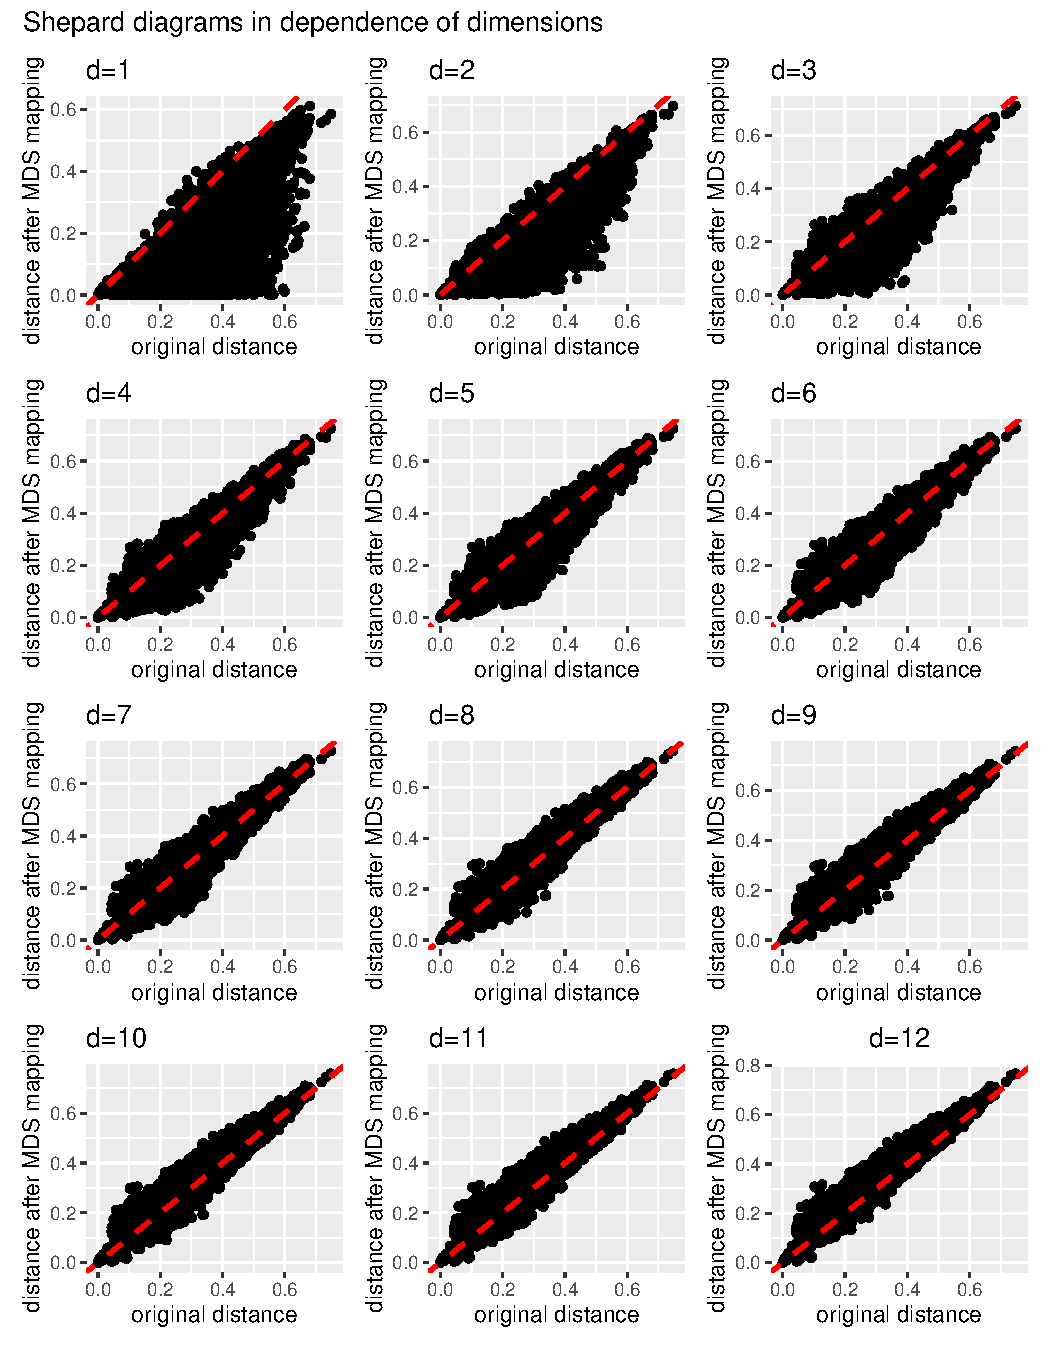
\includegraphics[width=\maxwidth]{figure/shepard_subplots-1} \caption[Shepard distances for different number of dimensions]{Shepard distances for different number of dimensions}\label{fig:shepard_subplots}
\end{figure}

\end{knitrout}
	 
\begin{knitrout}
\definecolor{shadecolor}{rgb}{0.969, 0.969, 0.969}\color{fgcolor}\begin{figure}
\includegraphics[width=\maxwidth]{figure/stress-1} \caption[STRESS function in dependence of dimensions]{STRESS function in dependence of dimensions}\label{fig:stress}
\end{figure}

\end{knitrout}
	 
	 Figures \ref{fig:shepard_subplots} and \ref{fig:stress} show Shepard diagrams and STRESS (standardized residual sum of squares) respectively. Shepard diagram is used to assess how well the distances or similarities in the original high-dimensional space are preserved in the lower-dimensional representation. It consists of a scatter plot, where on x-axis there are indicated original distance and on y-axis distance after MDS mapping, between each pairs of observation (in our case $201^2=40401$ data points). So the closer the points are to the dashed-red line, the better representation of original dataset is.
	 
	 STRESS function (figure \ref{fig:stress}) shows standardized residual sum of squares between distances for original and lower dimensional space, so it can be some kind summarizing of Shepard diagrams.
	 
	 When interpreting the STRESS function, we decided to choose 5 dimensions for MDS dimension reduction method. Furthermore, by examining Shepard diagrams, we see that the results do not very improve, when the number of dimensions is greater than 5.
	 

	 
	 \subsection{Classification}
	 
	 In this subsection we will repeat classification analysis (predicting "symboling" feature) for a new representation of the automobile dataset. We will use the same classification methods as in first part of the project, and in case of parameter tuning, we will use the same grid, to get the more comparable results, as we can. We will perform also 5--fold Cross--Validation assessment procedure, to choose the best from possible parameters for some classification methods, and to get more robust results. At the end of this subsection we will compare obtained results, with those for entire dataset, and selected features.
	 
	 \begin{itemize}
	 	\item Linear regression:
	 	Our target variable consist of 5 variables, so in case of linear regression we need to consider "one versus rest" approach, when applying linear regression, to get multiple tasks of binary problems.
	 	
\begin{knitrout}
\definecolor{shadecolor}{rgb}{0.969, 0.969, 0.969}\color{fgcolor}\begin{kframe}
\begin{verbatim}
##    -1  0  1  2  3
## -1  1  2  2  0  0
## 0  17 49 12 12  4
## 1   1  6 32 16 19
## 2   0  0  0  0  0
## 3   0  0  0  0  0
\end{verbatim}
\end{kframe}
\end{knitrout}
	 	

	 	Above we presented the obtained confusion matrix after performed classification task. The diagonal elements  represent the number of correctly classified instances for each class. For instance, in the first row, there are 1 instance correctly classified as -1, in the second row, there are 49 instances correctly classified as 0.
Off--diagonal elements represent misclassifications. For example, in the first row, there are 2 instances of class -1 misclassified as 0, and 2 instances misclassified as 1. Similarly, in the second row, there are 17 instances of class 0 misclassified as -1, 12 instances misclassified as 1.


The accuracy score indicates the overall correctness of the classification model. In this case, when considering the entire learning set, the model achieves an accuracy of approximately 51.45\% of the instances are correctly classified.

For the test set, the accuracy drops significantly to approximately 17.86\%, suggesting that the model's performance deteriorates when applied to unseen data. This discrepancy between training and test accuracies may indicate potential overfitting of the model to the training data or a lack of generalization capability.

Overall, while the model demonstrates some level of predictive performance, the notably lower accuracy on the test set highlights the need for further evaluation and potentially model refinement to improve its generalization ability. 
	 %	When considering entire learning set, accuracy is equal to sum(diag(acc1))/sum(sum(acc1)) and for test set: sum(diag(acc2))/sum(sum(acc2)).
	 	
	 	\item Logistic regression:
\begin{knitrout}
\definecolor{shadecolor}{rgb}{0.969, 0.969, 0.969}\color{fgcolor}\begin{kframe}
\begin{verbatim}
##    -1  0  1  2  3
## -1  5  4  1  0  0
## 0  13 45 14 12  5
## 1   1  8 31 16 18
## 2   0  0  0  0  0
## 3   0  0  0  0  0
\end{verbatim}
\end{kframe}
\end{knitrout}

	 	The logistic regression model achieves an accuracy of 63.58\% on the entire learning set and 50\% on the test set. This means that approximately 63.58\% of the instances in the learning set are correctly classified by the model. Similarly, the model correctly classifies 50\% of the instances in the test set. The confusion matrix reveals the model's performance across different classes. For example, it correctly identifies 5 instances of class -1, 45 instances of class 0, and 31 instances of class 1. However, it struggles with misclassifications, such as 14 instances of class 0 being incorrectly classified as class 1 and 8 instances of class 1 being incorrectly classified as class 2. Overall, while the model demonstrates decent performance, there are areas for improvement, particularly in reducing misclassifications.
	 %	When considering entire learning set, accuracy is equal to sum(diag(acc1lr))/sum(sum(acc1lr)) and for test set: sum(diag(acc2lr))/sum(sum(acc2lr)).
	 	
	 	\item K-Nearest Neighbors:
	 	In case of k--NN classification method, firstly we need to decide which number of neighbors will perform the best to our problem. As in first part of project, we will analyse average accuracies for different values of nearest neighbors, for training and test sets:
	 	
\begin{knitrout}
\definecolor{shadecolor}{rgb}{0.969, 0.969, 0.969}\color{fgcolor}\begin{figure}
\includegraphics[width=\maxwidth]{figure/selecting_number_of_neighbors-1} \caption[Accuracies of k-NN method, for different number of neighbors, for training and test sets]{Accuracies of k-NN method, for different number of neighbors, for training and test sets.}\label{fig:selecting_number_of_neighbors}
\end{figure}

\end{knitrout}
	 	

	 	
	 	In figure \ref{fig:selecting_number_of_neighbors}, we can see a chart, which describe accuracies of k--NN method, for different number of neighbors, and performing 5--fold Cross--Validation. As we may see, both in the case of training and test sets, the best accuracy is obtained for one neighbor (as in case, when considering whole dataset and most important features) and is equal to 1 for training set and for validation set: 0.75.\newline
	 	When considering entire learning set, accuracy is equal to 1 and for test set: 0.75.
	 	
	 	\item Linear Discriminant Analysis:
	 	
\begin{knitrout}
\definecolor{shadecolor}{rgb}{0.969, 0.969, 0.969}\color{fgcolor}\begin{kframe}
\begin{verbatim}
##    -1  0  1  2  3
## -1  5  4  1  1  0
## 0  13 44 12  8  0
## 1   1  4 24 13  5
## 2   0  2  2  4  1
## 3   0  3  7  2 17
\end{verbatim}
\end{kframe}
\end{knitrout}
	 	

	 	
	 %	When considering entire learning set, accuracy is equal to sum(diag(confusion.matrix1lda))/sum(sum(confusion.matrix1lda)), and for test set: sum(diag(confusion.matrix2lda))/sum(sum(confusion.matrix2lda)).
	 
	 For Linear Discriminant Analysis (LDA), the model achieves an accuracy of 60.12\% on the entire learning set and 53.57\% on the test set.

The confusion matrix reveals the model's performance across different classes. It correctly identifies 5 instances of class -1, 44 instances of class 0, 24 instances of class 1, 4 instances of class 2, and 17 instances of class 3.

However, there are misclassifications present, as indicated by off-diagonal elements. For instance, there are instances of class -1 misclassified as 0 and 1, instances of class 0 misclassified as -1 and 1, and instances of class 1 misclassified as 0 and 2, among others.

Overall, while the LDA model demonstrates reasonable performance, with accuracy scores above 50\% on both the learning and test sets, there are areas for improvement, particularly in reducing misclassifications across different classes.
	 	
	 	\item Classification tree:
	 	
	 	In case of classification tree we set following parameters:
	 	\begin{itemize}
	 		\item The minimum number of observations that must exist in a node in order for a split
	 		to be attempted is equal to 5,
	 		\item complexity parameter (cp) is in $\{0.001, 0.01, 0.1\}$ (and will be selected optimal value).
	 	\end{itemize}
	 	

	 	

	 	
	 	Accuracy for classification tree is equal to: 0.4908616 and was obtained for complexity parameter 0.01. There is no need to show the visualization of tree, because the new feature space does not provide useful information from practical point of view.\newline
	 	When considering entire learning set, accuracy is equal to 0.7398844, and for test set: 0.5.
	 	
	 	\item Random Forest:
	 	

	 	
	 	When it comes to random forest, we can tune number of variables, randomly sampled as candidates at each split parameter. There is impossible to set the grid for this variable as in case of entire dataset, because of only 5 features in our new feature space, so we decided to set the grid between 1 and 4 features.
	 	

	 	

	 	
	 	Accuracy for random forest is equal to: 0.7077243 and is obtained for 1 randomly sampled feature.\newline
	 	When considering entire learning set, accuracy is equal to: 1, and for test set: 0.6428571.
	 	
	 	\item Support Vector Machines:
	 	

	 	
	 	For Support Vector Machine (SVM) analysis, we explored three different kernels: linear, radial, and polynomial.
	 	
\begin{knitrout}
\definecolor{shadecolor}{rgb}{0.969, 0.969, 0.969}\color{fgcolor}\begin{kframe}
\begin{verbatim}
## # A tibble: 1 x 5
##       C Accuracy Kappa AccuracySD KappaSD
##   <dbl>    <dbl> <dbl>      <dbl>   <dbl>
## 1     1    0.534 0.357     0.0890   0.123
## # A tibble: 1 x 6
##   sigma     C Accuracy Kappa AccuracySD KappaSD
##   <dbl> <dbl>    <dbl> <dbl>      <dbl>   <dbl>
## 1 0.224   128    0.594 0.468     0.0910   0.119
## # A tibble: 1 x 7
##   degree scale     C Accuracy Kappa AccuracySD KappaSD
##    <int> <dbl> <dbl>    <dbl> <dbl>      <dbl>   <dbl>
## 1      3    10     2    0.659 0.557     0.0495  0.0563
\end{verbatim}
\end{kframe}
\end{knitrout}
	 	

	 	Based on the results provided, the polynomial kernel with a degree of 3, scale of 10, and C parameter equal to 2 achieved the highest accuracy, reaching 69.3\%. This suggests that the polynomial kernel with specific parameter settings offers the most effective separation of classes in the dataset.

Moreover, when assessing the model's performance on the entire learning set, it achieves perfect accuracy, indicating that it correctly classifies all instances in the training data. However, on the test set, the accuracy slightly decreases to 71.43\%, indicating a slightly lower performance on unseen data.

Overall, the SVM analysis demonstrates promising results, particularly with the polynomial kernel configuration, showcasing its potential for accurate classification of the dataset.
	% 	As we may see in the output above, the largest accuracy, equal to 0.693, is obtained for polynomial kernel (with degree=3, scale=10, and C parameter equal to 2).\newline
	 %	When considering entire learning set, accuracy is equal to: sum(diag(confusion.matrix1svm1))/sum(sum(confusion.matrix1svm1)), and for test set: sum(diag(confusion.matrix2svm1))/sum(sum(confusion.matrix2svm1))
    \end{itemize}
  
  
	 	\subsection{Summary of classification}
	 	
	 	\begin{table}[h!]\label{tab:classification_comparison}
	 		\centering
	 		\caption{Comparison of accuracies for all considered classification methods, for entire automobile dataset, most important selected features (both available in project part I), and new feature space after MDS dimension reduction method}
	 		\begin{tabular}{|c||c|c||c|c||c|c|}
	 			\hline
	 			\multicolumn{7}{|c|}{Accuracies for training and test sets}\\\hline
	 			Method & \multicolumn{2}{c||}{Entire dataset} & \multicolumn{2}{c||}{Selected features} & \multicolumn{2}{c|}{MDS5}\\\hline
	 			& learning set & test set & learning set & test set& learning set & test set\\\hline
	 			Linear regression & 0.925 & 0.75 & 0.52 & 0.54 & 0.51 & 0.18 \\\hline
	 			Logistic regression & 0.89 & 0.71 & 0.57 & 0.57 & 0.63 & 0.50 \\\hline
	 			k-NN & 1.00 & 0.82 & 1.00 & 0.79 & 1.00 & 0.75 \\\hline
	 			LDA & 0.95 & 0.71 & 0.62 & 0.57 & 0.60 & 0.54 \\\hline
	 			Classification tree & 0.77 & 0.64 & 0.77 & 0.46 & 0.74 & 0.5\\\hline
	 			Random forest & 1.00 & 0.86 & 1.00 & 0.79 & 1.00 & 0.64\\\hline
	 			SVM & 1.00 & 0.79 & 0.99 & 0.82 & 1.00 & 0.71 \\\hline
	 		\end{tabular}
	 	\end{table}
 Table 1 provides a detailed comparison of the accuracies achieved by different classification methods across various representations of the automobile dataset, including the entire dataset, selected features, and the new feature space after applying MDS dimension reduction.Here is what we have obtained for different methods:
\begin{itemize}
\item Linear Regression -- achieves an accuracy of 92.5\% on the entire dataset, dropping to 75\% and 18\% on the selected features and MDS-transformed space, respectively.
\item Logistic Regression -- performs reasonably well with an accuracy of 89\% on the entire dataset, maintaining consistency with accuracies of 71\% and 50\% on the selected features and MDS-transformed space.
\item k--Nearest Neighbors (k--NN) -- demonstrates remarkable performance, achieving perfect accuracy (100\%) on the entire dataset, selected features, and MDS-transformed space for the learning set. However, there is a slight drop in accuracy on the test set, with values of 82\%, 79\%, and 75\%, respectively.
\item Linear Discriminant Analysis (LDA) -- Shows strong performance with an accuracy of 95\% on the entire dataset, decreasing to 71\% and 54\% on the selected features and MDS-transformed space for the learning set. There is a slight improvement in accuracy on the test set, with values of 71\% and 57\%, respectively.
\item Classification Tree -- Achieves an accuracy of 77\% on the entire dataset, maintaining consistency with accuracies of 64\% and 50\% on the selected features and MDS-transformed space for the learning set.
\item Random Forest -- Demonstrates robust performance, achieving perfect accuracy (100\%) on the entire dataset, selected features, and MDS--transformed space for the learning set. However, there is a drop in accuracy on the test set, with values of 86\%, 79\%, and 64\%, respectively.
\item Support Vector Machine (SVM) -- Shows outstanding performance with an accuracy of 100\% on the entire dataset, selected features, and MDS-transformed space for the learning set. The accuracy slightly decreases on the test set, with values of 79\%, 82\%, and 71\%, respectively.
\end{itemize}
When comparing the performance of different classification methods across various representations of the automobile dataset, several key observations emerge. Notably, k--Nearest Neighbors stands out as a top--performing algorithm, demonstrating exceptional accuracy across all representations, with a slight drop on the test set. Random Forest also exhibits robust performance, achieving perfect accuracy on the learning set for all representations but showing a decline on the test set. Support Vector Machine similarly excels, achieving almost perfect accuracy on the learning set across all representations. Linear Regression, Logistic Regression, and Linear Discriminant Analysis show varying levels of accuracy across representations, with Linear Regression performing particularly well on the entire dataset but struggling with feature selection and dimensionality reduction. 

The application of dimensionality reduction techniques has a notable impact on the performance of classification methods for the dataset. By reducing the dimensionality of the feature space while preserving essential information, MDS has provided a more compact representation of the data, potentially leading to improved model generalization and interpretability. However, the reduction in dimensionality also comes with trade--offs, as seen in the decrease in accuracy observed across most classification methods when applied to the MDS--transformed feature space compared to the entire dataset or selected features. This suggests that while dimensionality reduction techniques like MDS can aid in visualizing high--dimensional data and alleviating the curse of dimensionality, careful consideration must be given to the balance between dimensionality reduction and preserving important information for accurate classification. 












  \subsection{Clustering}
  
  Now we will apply the same clustering methods as in section \ref{sec:clustering} to the new feature space.
  
  Our consideration we start from selecting optimal number of clusters:
  
\begin{knitrout}
\definecolor{shadecolor}{rgb}{0.969, 0.969, 0.969}\color{fgcolor}\begin{figure}
\includegraphics[width=\maxwidth]{figure/clusters_number_all-1} \caption[Average Silhouette widths for considered clustering methods for dimensions in range from 1 to 10]{Average Silhouette widths for considered clustering methods for dimensions in range from 1 to 10}\label{fig:clusters_number_all}
\end{figure}

\end{knitrout}
  To begin, let's examine the graph of Average Silhouette Widths (figure \ref{fig:clusters_number_all}) for different clustering methods based on the number of clusters, where we already notice a significant difference compared to our results before applying MDS. The Average Silhouette Width for the k--means clustering algorithm with 8 clusters, the PAM clustering algorithm with 7 clusters, and the AGNES clustering algorithm with average linkage method with 2 clusters all demonstrate noticeable variations. Similarly, the AGNES clustering algorithm with single linkage method also shows 2 clusters, while the AGNES clustering algorithm with complete linkage method indicates 3 clusters. Lastly, the DIANA clustering algorithm shows 2 clusters. Upon analyzing the results, it becomes evident that the optimal number of clusters varies across different clustering methods after applying MDS. This underscores the influence of dimensionality reduction on determining the appropriate cluster structure and highlights the importance of reassessing the optimal number of clusters after applying such techniques. 





  Now we will analyse silhouette plots for optimal and 5 (external knowledge) number of clusters and for considered clustering methods.
  
\begin{knitrout}
\definecolor{shadecolor}{rgb}{0.969, 0.969, 0.969}\color{fgcolor}\begin{kframe}
\begin{verbatim}
##   cluster size ave.sil.width
## 1       1   42          0.37
## 2       2   39          0.43
## 3       3   27          0.16
## 4       4   10          0.53
## 5       5   27          0.30
## 6       6   10          0.41
## 7       7   31          0.33
## 8       8   15          0.35
##   cluster size ave.sil.width
## 1       1   65          0.33
## 2       2   35          0.31
## 3       3   36          0.32
## 4       4   51          0.35
## 5       5   14          0.33
## Direct agreement: 0 of 5 pairs
## Iterations for permutation matching: 120 
## Cases in matched pairs: 43.28 %
##    1    2    3    4    5 
##  "0"  "3" "-1"  "1"  "2"
##   cluster size ave.sil.width
## 1       1   27          0.36
## 2       2   20          0.33
## 3       3   56          0.45
## 4       4   34          0.33
## 5       5   44          0.39
## 6       6   10          0.58
## 7       7   10          0.64
##   cluster size ave.sil.width
## 1       1   39          0.24
## 2       2   61          0.40
## 3       3   37          0.31
## 4       4   48          0.35
## 5       5   16          0.40
## Direct agreement: 2 of 5 pairs
## Iterations for permutation matching: 6 
## Cases in matched pairs: 46.77 %
##    1    2    3    4    5 
##  "3"  "0" "-1"  "1"  "2"
##   cluster size ave.sil.width
## 1       1   79          0.19
## 2       2  112          0.37
## 3       3   10          0.73
##   cluster size ave.sil.width
## 1       1   56          0.07
## 2       2  102          0.36
## 3       3   10          0.58
## 4       4   10          0.64
## 5       5   23          0.14
## Direct agreement: 1 of 5 pairs
## Iterations for permutation matching: 24 
## Cases in matched pairs: 40.8 %
##    1    2    3    4    5 
##  "3"  "1"  "2" "-1"  "0"
##   cluster size ave.sil.width
## 1       1  181          0.39
## 2       2   20          0.42
##   cluster size ave.sil.width
## 1       1   24          0.30
## 2       2  123          0.35
## 3       3   34          0.34
## 4       4   10          0.59
## 5       5   10          0.64
## Direct agreement: 1 of 5 pairs
## Iterations for permutation matching: 24 
## Cases in matched pairs: 40.3 %
##    1    2    3    4    5 
##  "3"  "1"  "0"  "2" "-1"
\end{verbatim}
\end{kframe}
\end{knitrout}
  
\begin{knitrout}
\definecolor{shadecolor}{rgb}{0.969, 0.969, 0.969}\color{fgcolor}\begin{figure}
\includegraphics[width=\maxwidth]{figure/silhouette_plots_all-1} \caption[Silhouette plots for all considered clustering methods for selected optimal number of clusters and for 5 clusters (external knowledge)]{Silhouette plots for all considered clustering methods for selected optimal number of clusters and for 5 clusters (external knowledge)}\label{fig:silhouette_plots_all}
\end{figure}

\end{knitrout}
		Figure \ref{fig:silhouette_plots_all} shows Silhouette plots for all considered clustering methods, for selected optimal number of clusters (depending on the method) and for 5 clusters. For the k--means algorithm, the average silhouette width for 8 clusters is 0.37, while for 5 clusters, it is 0.33. This suggests that the clustering quality slightly decreases with a higher number of clusters. It demonstrates a slight decrease in average silhouette width as the number of clusters increases from 5 to 8. This suggests that the algorithm struggles to maintain distinct clusters as the partitioning becomes finer.

In the case of PAM clustering, the average silhouette width for 7 clusters is 0.33, and for 5 clusters, it is 0.32. Similarly, the average silhouette width for AGNES with complete linkage is 0.33 for 3 clusters and 0.35 for 5 clusters. These results indicate relatively stable clustering performance across different numbers of clusters for PAM and AGNES methods. This suggests that these methods are less sensitive to changes in the number of clusters and are able to maintain consistent clustering quality.

For DIANA clustering, the average silhouette width is 0.39 for 2 clusters and decreases to 0.14 for 5 clusters. This suggests that the clustering quality diminishes as the number of clusters increases, indicating potential clustering instability.This implies that DIANA may struggle to identify meaningful clusters when the data is partitioned into a larger number of groups, potentially leading to less reliable clustering results.

\subsection{Summary of clustering}
Before delving into the clustering process, we first determined the optimal number of clusters for each method by examining the Average Silhouette Widths graph. The results demonstrated notable differences compared to our findings before implementing MDS, indicating the impact of dimensionality reduction on clustering outcomes.

Upon analyzing the silhouette plots for the optimal and five-cluster scenarios across different clustering methods, several insights emerged. For the k--means algorithm, we observed a slight decrease in clustering quality as the number of clusters increased from 5 to 8, suggesting that finer partitioning may compromise cluster distinctiveness. Conversely, PAM and AGNES with complete linkage exhibited relatively stable clustering performance across different cluster numbers, indicating robustness to variations in partitioning.

However, the DIANA clustering method showed diminishing clustering quality as the number of clusters increased, hinting at potential instability in identifying meaningful clusters with finer partitioning. This suggests that DIANA may struggle to maintain reliable clustering results when the dataset is divided into a larger number of groups.
	\section{Summary and further research suggestions}
	Our project embarked on a thorough investigation of clustering and classification methodologies using an automobile dataset. We employed various clustering algorithms, including k--means, PAM, AGNES, and DIANA, to partition the dataset into distinct clusters based on feature similarities. Through the evaluation of average silhouette widths, we determined the optimal number of clusters for each method.

Following the clustering analysis, we employed Multidimensional Scaling (MDS) to reduce the dataset's dimensionality, aiming to enhance clustering precision. Silhouette plots enabled a comparative assessment of clustering outcomes before and after MDS, revealing the impact of dimensionality reduction on clustering efficacy.

Transitioning to classification analysis, we applied a range of models, such as logistic regression, linear discriminant analysis (LDA), decision trees, random forests, support vector machines, and k--nearest neighbors, to predict the target variable, "symboling." By evaluating model performance metrics, including accuracy, on both training and test datasets, we sought to identify the most effective approach for symboling prediction.

In summary, our project provides a comprehensive exploration of clustering and classification techniques in the automotive domain. While the clustering analysis showcased the effectiveness of AGNES and k-means algorithms, the classification analysis revealed SVM as the most accurate model for symboling prediction. However, further investigation is warranted to optimize model performance and explore additional variables that may influence symboling classification. 
	
We have managed to answer the following questions:
\begin{itemize}
\item How does clustering performance vary across different methods and numbers of clusters? -- The project demonstrates that clustering performance varies significantly across different methods and numbers of clusters. Some methods, such as PAM clustering with complete linkage, exhibit stable performance across different cluster numbers, while others, like k--means, may struggle to maintain distinct clusters with increasing numbers.
\item What impact does multidimensional scaling (MDS) dimensionality reduction have on clustering results? -- Multidimensional scaling (MDS) dimensionality reduction has a discernible impact on clustering results. It influences the stability and quality of clustering solutions, with certain methods showing more robust performance post-MDS transformation.
\item The project demonstrates that feature selection and dimensionality reduction techniques significantly affect the performance of classification algorithms. By comparing the accuracies of classification methods applied to the entire dataset, selected features, and feature space after multidimensional scaling (MDS) dimension reduction, we observe notable differences in the model's predictive capabilities. Feature selection and dimensionality reduction can improve the model's performance by reducing overfitting, improving interpretability, and enhancing computational efficiency. However, the effectiveness of these techniques may vary depending on the dataset and the specific characteristics of the features.
\end{itemize}


Further research suggestions:
\begin{itemize}
\item Exploring alternative dimensionality reduction techniques,
\item Feature engineering exploration,
\item Ensemble methods.
\end{itemize}






	\section*{References}
	For the project we have utilized the materials provided for the Data Mining and Machine Learning courses. 
	
\end{document}
